\documentclass{article}
\usepackage{fullpage}
\usepackage{amssymb}
\usepackage{amsmath}
\usepackage{amsfonts}
\usepackage{mathrsfs}
\usepackage{graphicx}
\author{Anthony LaTorre}
\date{\today}
\title{Some thoughts on SNO+ Reconstruction}

\newcommand{\like}{\mathscr{L}}
\newcommand{\N}{\mathrm{N}}
\begin{document}
\maketitle
\section{Energy}
We can estimate a lower limit to the energy resolution of SNO+ by imagining a
likelihood analysis independent of the position of the event, which depends
only on the number of detected photons $\N$. The likelihood function $\like$
is given by:

\begin{equation}
    \like(E) \equiv P(\N|E) = \sum_{j \geq \N} \sum_{k \geq j} P(j|E) P(k|j) P(\N|k)
    \label{energy_likelihood}
\end{equation}

where $j$ is the number of photons created, $k$ is the number of photons that
reach a PMT, and $\N$ is the number of photons detected. The number of photons
created follows a Poisson distribution

\[
    P(j|E) = e^{-\mu} \frac{\mu^j}{j!}
\]

where $\mu$ is usually assumed to depend linearly on the energy $E$.

For isotropic light, the number of photons reaching the PMTs, $k$, follows a
binomial distribution:

\[
    P(k|j) = \binom{k}{j} p^j (1-p)^{k-j}
\]

where $p$ is the probability that any one photon hits a PMT. For an event at
the center, $p$ would be equal to the coverage of the detector. The probability
that $\N$ photons are then detected out of the $k$ that hit a PMT also follows a
binomial distribution with $p$ being the quantum efficiency of the PMT (I'll
call it $q$).

The sum in Equation~\ref{energy_likelihood} reduces to a single Poisson distribution

\[
    \like(E) = e^{-\lambda} \frac{\lambda^\N}{\N!}
\]

with a mean $\lambda$ equal to the product of $p$, $q$, and $\mu$. We know from
simulations that $\lambda$ is approximately equal to 400 hits per MeV.

We can estimate the resolution by looking at the standard deviation of the
likelihood function for a given $\N$.

\[
    \mathbb{E}(\lambda) = \int \lambda \like(E) = \N+1
\]
\[
    \mathbb{E}(\lambda^2) = \int \lambda^2 \like(E) = (\N+2)(\N+1)
\]

\[
    \mathrm{Var}(\lambda) = \mathbb{E}(\lambda^2) - \mathbb{E}(\lambda)^2 = \N + 1
\]

Therefore, we see that the energy resolution $\sigma$ is given by

\[
    \sigma = \frac{\sqrt{\N+1}}{400}
\]

For a 3 MeV event, the lowest achievable energy resolution is therefore around
0.09 MeV, or 3\%.

\section{Position Reconstruction}

We can try a similar method to estimate a lower limit to the position
resolution achievable in SNO+. For simplicity, assume a perfectly spherical
detector and only direct light, without any spread in time due to the PMTs.
Scintillation light typically contains multiple components, each component
emitting light with a different time constant. For the purpose of estimating a
lower bound on the position resolution, I will assume the light only comes from
a single component. In this case the likelihood can be written as
\cite{mccarty},

\[
    \like(\mathbf{x}) = \prod_i e^{-(t - t_0 - s_i)}
    \frac{\cos{\phi}}{4 \pi s_i^2}
\]

where $s_i$ is equal to the distance between the proposed event $\mathbf{x}$ and
the PMT $\mathbf{x_i}$, and $\phi$ is the angle between the normal of the
sphere and the vector $\mathbf{s_i}$. In reference~\cite{mccarty}, McCarty
estimates the position resolution by assuming a \emph{gaussian} time profile of
emission, and finding the second derivative of the likelihood function at the
maximum, and obtains

\begin{equation}
    \sigma \approx \sqrt{\frac{3}{\N}} \frac{c \tau}{n}
    \label{gauss_sigma}
\end{equation}

where $n$ is the refractive index of the scintillator material, and $\N$ is the
number of hits detected. For SNO+, this estimate gives a resolution of 5 cm for
a 3 MeV event.

To verify this, I wrote a simple Monte Carlo simulation and fit for the
position of an event generated at the center of the detector for different $\N$.
A plot of the resolution as a function of $\N$ is shown in Figure~\ref{res_n}.

\begin{figure}[h!]
    \centering
    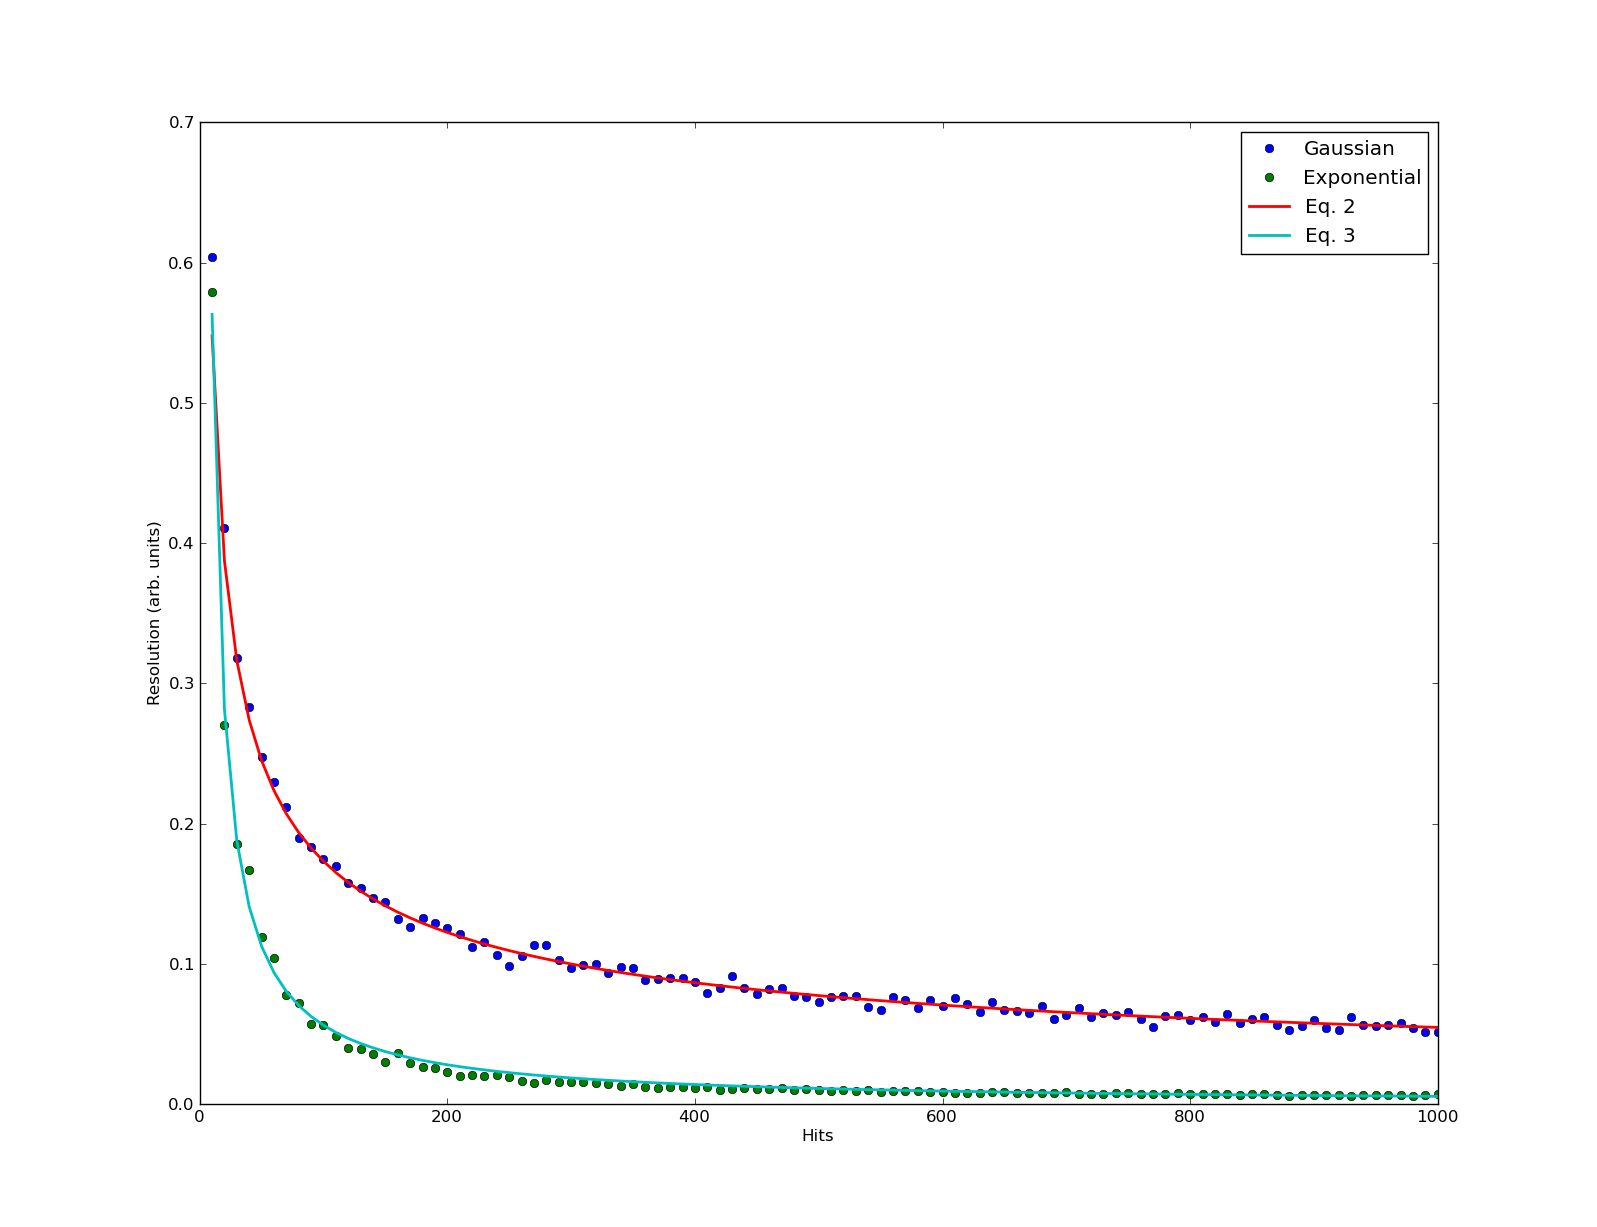
\includegraphics[width=0.85\linewidth]{gauss_exp2.png}
    \caption{Resolution vs. Hits}
    \label{res_n}
\end{figure}

The gaussian time profile case is modeled well by the formula in
Equation~\ref{gauss_sigma}, but the resolution for the exponential time profile
is much better! The exponential resolution is modeled best by

\begin{equation}
    \sigma \approx \frac{5.63}{\N} \frac{c \tau}{n}
\end{equation}

This would predict a lower limit for position resolution at 0.5 cm for a 3 MeV
event. To check that the fitter I wrote was actually fitting events correctly,
I made a pull plot, shown in Figure~\ref{pull_plot}. It fits well to a standard
normal distribution and so I have confidence that these results are meaningful.
In order to understand this difference, I think it's instructive to consider
the one dimensional case.

\begin{figure}[h!]
    \centering
    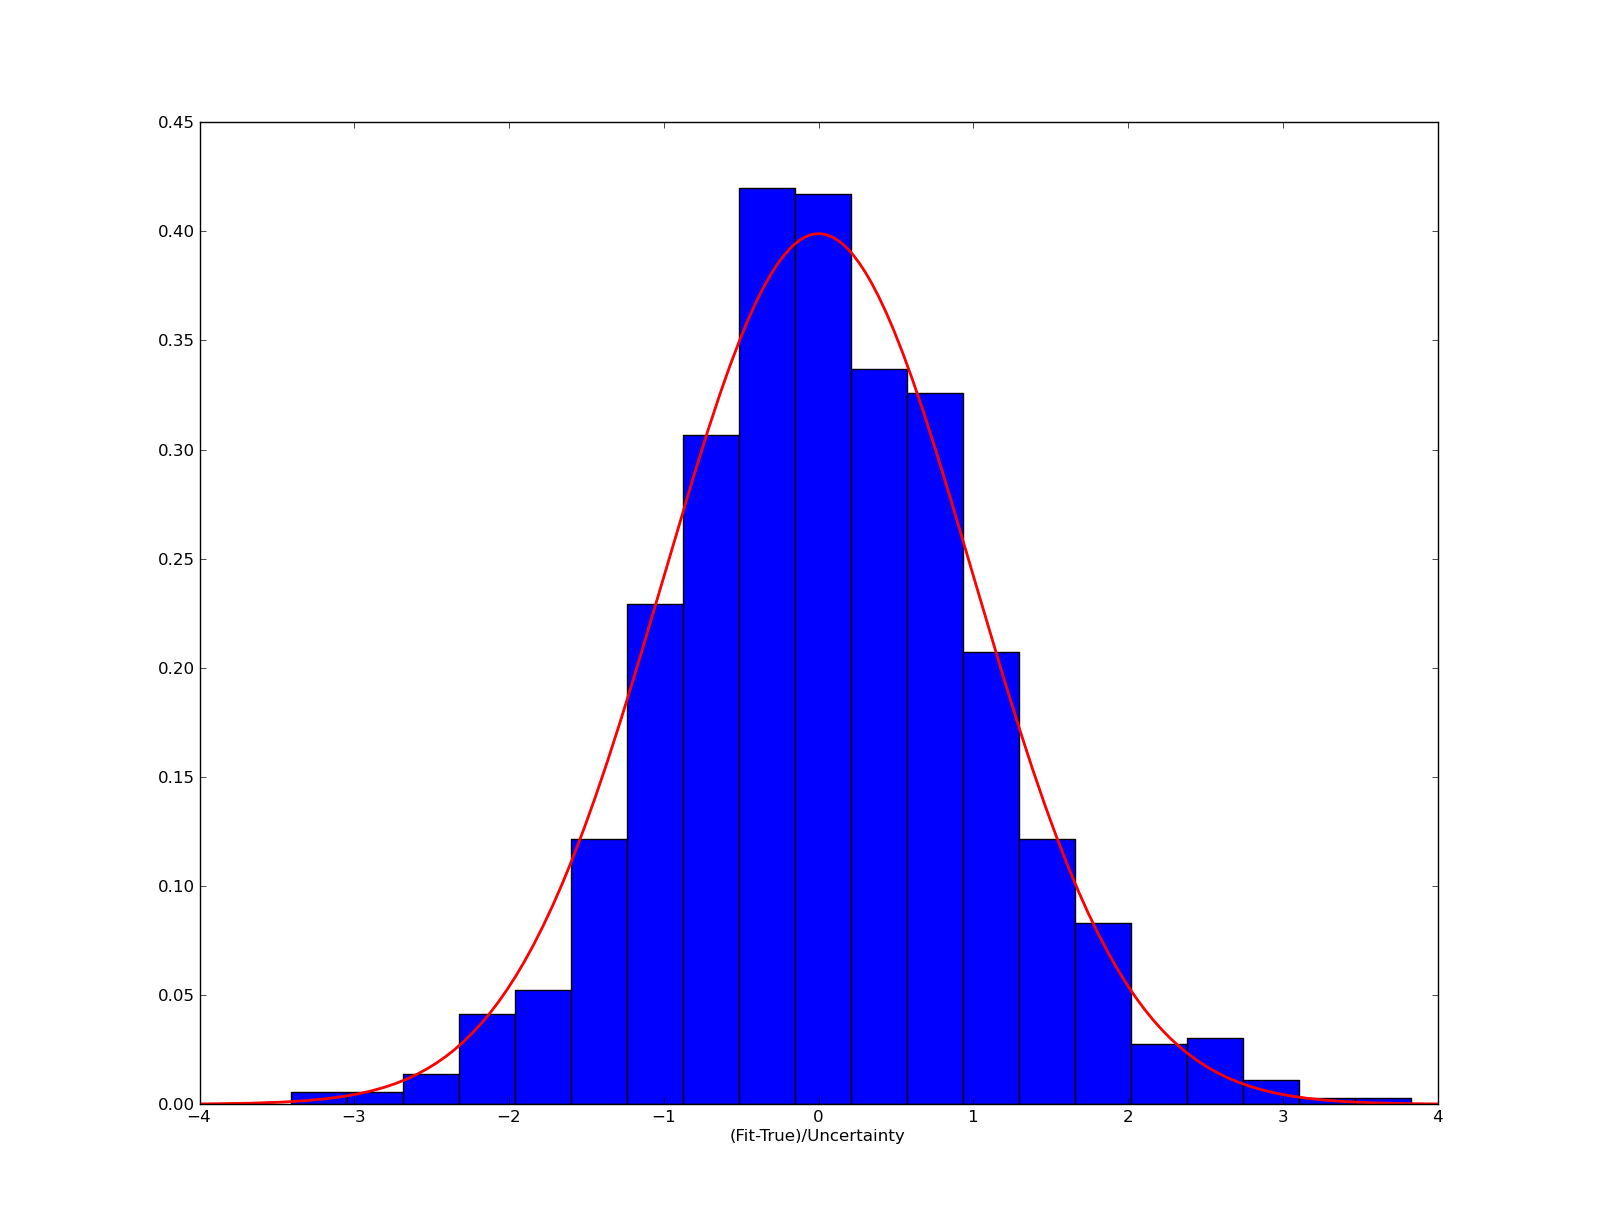
\includegraphics[width=0.85\linewidth]{pull_plot.png}
    \caption{Pull Plot}
    \label{pull_plot}
\end{figure}

\subsection{1D Position Reconstruction}

In the one dimensional case, assume we have a single PMT with perfect timing,
and we want to estimate the distance to some scintillation event.

\subsubsection{Gaussian Time Profile}
If the light is emitted with a Gaussian time distribution, we can estimate the
position by maximizing the likelihood

\[
    \like(x) = \prod_i e^{-\frac{(t_i-x)^2}{2 \tau^2}}
\]

We can find the maximum by setting the first derivative to 0,

\[
    \frac{d\like}{dx} = -\left(\sum_i \frac{t_i - x}{\tau^2} \right) \prod_i
    e^{-\frac{(t-x)^2}{2 \tau^2}} = 0
\]

The maximum is therefore simply the mean of the times

\[
    \hat{x} = \frac{1}{\N} \sum_i t_i
\]

The resolution at the maximum is found easiest by expanding $\log{\like}$ in a
Taylor series about the maximum.

\[
    \log{\like} = - \sum_i \frac{(t_i-x)^2}{2 \tau^2}
\]

\[
    \frac{d^2\like(\hat{x})}{dx^2} = -\frac{\N}{\tau^2}
\]

Therefore,

\[
    \log{\like} \approx \mathrm{const} - \frac{\N}{\tau^2} x^2
\]

and

\[
    \like \approx e^{-\frac{\N}{\tau^2} x^2}
\]

from which, the resolution $\sigma$ is given by

\[
    \sigma = \frac{\tau}{\sqrt{\N}}
\]

\subsubsection{Exponential Time Profile}

The case of light emitted with an exponential time distribution can be treated
in a similar manner. The likelihood function is given by

\[
    \like = \prod_i e^{-\frac{t_i - x}{\tau}}
\]

In this case however, the best estimate for $x$ is given by

\[
    x = \min{t_i}
\]

The resolution is therefore found from the distribution for the smallest value
selected from $\N$ exponentially distributed numbers. This distribution is
simply an exponential with mean $\frac{\N}{\tau}$ \cite{order}.

Therefore, the resolution is given by

\[
    \sigma = \frac{\tau}{\N}
\]

The resolution scales with $\N$ and \emph{not} $\sqrt{\N}$ like in the Gaussian
case.

\begin{thebibliography}{9}
\bibitem{mccarty} Kevin McCarty,
\emph{The Borexino Nylon Film and the Third Counting Test Facility}.
Chapter 5.

\bibitem{order} Kyle Siegrist,
\emph{http://www.math.uah.edu/stat/sample/OrderStatistics2.html}
\end{thebibliography}

\end{document}
